\documentclass[aspectratio=169,10pt]{beamer}

\usetheme{Madrid}
\usecolortheme{default}

\usepackage[UTF8]{ctex}
\usepackage{booktabs}
\usepackage{tabularx}
\usepackage{xcolor}
\usepackage{tikz}
\usepackage{graphicx}
\usepackage{array}
\usepackage{colortbl}

\usetikzlibrary{arrows.meta,positioning,fit}

\definecolor{MainBlue}{RGB}{40,82,145}
\definecolor{AccentRed}{RGB}{178,56,46}
\definecolor{SoftGray}{RGB}{245,247,250}
\definecolor{DarkGray}{RGB}{70,76,86}

\setbeamercolor{title}{fg=MainBlue}
\setbeamercolor{frametitle}{fg=white}
\setbeamercolor{block title}{bg=MainBlue,fg=white}
\setbeamercolor{block body}{bg=SoftGray,fg=black}
\setbeamercolor{alerted text}{fg=AccentRed}
\setbeamertemplate{navigation symbols}{}
\setbeamertemplate{footline}{}
\setbeamertemplate{headline}{}
\newcommand{\keypoint}[1]{\textbf{\textcolor{AccentRed}{#1}}}
\newcommand{\bluepoint}[1]{\textbf{\textcolor{MainBlue}{#1}}}

\title{KVState: Persistent State Management for Multi-Turn Long-Context LLM Serving}
\author{}
\date{}

\begin{document}

\begin{frame}[plain]
\centering
\vspace{2.2em}

{\fontsize{26pt}{31pt}\selectfont\textbf{\textcolor{MainBlue}{KVState}}}

\vspace{0.9em}

{\Large\textbf{Persistent State Management for\\ Multi-Turn Long-Context LLM Serving}}

\vspace{1.5em}

{\large\textbf{面向多轮长上下文服务的持久化 KV 状态管理系统}}

\vfill

{\small KV is not merely a cache; it is persistent serving state.}

\end{frame}

\begin{frame}[t]{What Is the Problem?}
\small
\vspace{-0.5em}

\textbf{\textcolor{MainBlue}{背景：Agent 与科学发现推理正在将上下文长度推向 1M tokens}}

\vspace{0.2em}
在生产级长上下文推理中，历史上下文会在 prefill 阶段形成 KV 状态，这些状态需要在后续多轮请求的 prefill 与 decode 中持续、准确地复用。随着上下文长度扩展到 128K 乃至 1M tokens，KV 已不再是单次请求内的临时缓存，而是随会话、文档和工具轨迹持续增长的服务状态。

\vspace{0.8em}

\begin{beamercolorbox}[wd=\linewidth,sep=0.7em,rounded=true]{block body}
\textbf{\textcolor{AccentRed}{核心问题：}}
% 当可复用 KV 状态的规模超过 GPU 显存容量时，现有前缀缓存和 KV 卸载机制难以有效支撑此类工作负载：推理引擎内的热缓存通常不具备跨会话持久性，而基于 SSD 的按需取回机制可能在 prefill 或 decode 的关键路径上引入阻塞。

现有工作通过引擎内前缀缓存、外部 KV 存储以及基于 SSD 的数据搬移来改善 KV 复用，但它们仍然对一个关键的状态管理问题探索不足：当可复用的历史 KV 超出 GPU 显存时，冷 KV 对象虽然持久化保存，却并未处于可执行状态；若在预填充或解码阶段才去发现它，就可能将存储 I/O 转化为在线的尾部延迟。
\end{beamercolorbox}

\end{frame}

\begin{frame}[t]{Why Does It Matter?}
\vspace{0.35em}

\begin{block}{1、长上下文多轮对话正在成为 LLM 服务的重要形态}
企业级 RAG、代码助手和多智能体工作流通常围绕文档、代码库、任务状态和历史交互持续展开，而不是一次性问答。因此，系统性能瓶颈不再只来自单次请求计算，也越来越来自如何高效承载和复用长历史上下文。
\end{block}

\vspace{0.35em}

\begin{block}{2、KV 多级存储正在成为支撑长上下文服务的必要机制}
长上下文 KV 状态会随 token 数、模型层数和并发请求数快速增长，GPU 显存难以长期容纳所有可复用 KV。因此，将 KV 扩展到 CPU 内存和 SSD 等更大容量层级，是突破显存限制、降低重复 prefill 成本的重要方向。
\end{block}

\vspace{0.35em}

\begin{block}{3、KV 跨请求复用决定了多轮长上下文服务能否真正高效}
对于多轮 RAG、代码助手和 Agent 任务，后续请求往往会反复引用前序历史上下文。如果历史 KV 不能跨请求持久保存和准确复用，系统就只能反复重算相同上下文，导致 TTFT、吞吐和服务成本显著恶化。
\end{block}
\end{frame}

\begin{frame}[t]{Why Does Existing Work Fall Short? 为什么已有工作没有解决这个问题？}
\fontsize{6.8pt}{7.6pt}\selectfont
\vspace{-0.8em}

\setlength{\tabcolsep}{2.4pt}
\renewcommand{\arraystretch}{1.25}
\begin{tabularx}{\linewidth}{
>{\raggedright\arraybackslash}p{0.15\linewidth}
>{\centering\arraybackslash}p{0.20\linewidth}
>{\raggedright\arraybackslash}p{0.29\linewidth}
>{\raggedright\arraybackslash}X}
\rowcolor{gray!35}
\textbf{类别} & \textbf{代表方法} & \textbf{具体措施} & \textbf{关键不足} \\
\hline

GPU 内 KV 管理 &
PagedAttention, APC, RadixAttention &
将 KV 切块管理，并用哈希表或前缀树复用相同前缀，减少显存碎片和重复预填充。 &
主要解决 \textbf{HBM/CPU 内 KV 的管理与复用}；一旦历史 KV 超出容量并进入 SSD/外部冷层，就缺少持久化对象抽象、精确定位协议和恢复前 SLA 预算。 \\
\hline

PD 分离与跨实例 KV 传输 &
DistServe, Splitwise, NIXL connector, Mooncake &
分离预填充和解码实例，并在阶段之间传递 KV，降低资源干扰。 &
主要解决 \textbf{prefill/decode 阶段隔离与跨实例 KV 传输} 问题，没有将长期历史 KV 建模为可索引、可恢复、可准入控制的服务状态。 \\
\hline

外部 KV 缓存层 &
LMCache, Mooncake &
在推理引擎外维护 KV 缓存，支持跨请求、跨实例复用，并扩展到主存或 SSD。 &
主要解决 \textbf{显存扩容与跨请求复用} 问题，没有在请求进入模型前显式检查所需历史 KV 是否就绪，也缺少冷 KV 先恢复、再执行的准入机制。 \\
\hline

冷层存储与恢复调度 &
Tutti, CacheFlow, DualPath, FlexGen, Infinite-LLM, KVDrive &
从主存、SSD 或远端存储恢复 KV，并用流水、并行和调度隐藏 I/O。 &
主要回答 \textbf{冷层 KV 数据搬运与 I/O 隐藏}，但重点在于优化“如何搬得更快、如何与计算重叠”，而不是在请求进入模型前显式判断其历史 KV 依赖是否就绪，并据此做等待、恢复、重算或准入决策。 \\
\hline

文档片段复用 &
CacheBlend, RAGCache &
面向 RAG 或多文档场景复用共享文档、chunk 或非严格前缀 KV，通过融合或选择性重算降低 TTFT。 &
主要解决 \textbf{RAG 文档片段或非严格前缀的 KV 局部复用} 问题，但没有将已提交的多轮历史 KV 作为长期状态，持续追踪其位置、冷热状态和执行前可用性。 \\
\hline

近似、压缩与驱逐 &
H2O, Scissorhands, CacheGen, TTKV &
通过压缩、量化或重要性筛选降低 KV 容量和带宽开销。&
主要解决 \textbf{KV 容量压缩、传输编码和缓存驱逐} 问题，关注的是如何减少 KV 本身的成本，而不是如何对已提交历史 KV 进行精确状态追踪、冷层恢复和执行前准入控制。 \\
\end{tabularx}

\vspace{0.35em}
\begin{beamercolorbox}[wd=\linewidth,sep=0.5em,rounded=true]{block body}
\textbf{\textcolor{AccentRed}{总结：}}
已有工作分别优化热前缀复用、跨实例 KV 传输和多级存储数据搬运；
但它们大多没有将长期历史 KV 建模为
\textbf{可持久化、可索引、可恢复、可准入控制的 serving state}。
因此，面对多轮长上下文服务，系统仍缺少执行前的历史 KV 就绪检查与准入机制，
难以稳定避免重复 prefill 或将冷数据恢复暴露到在线执行路径。
\end{beamercolorbox}

\end{frame}

\begin{frame}[t]{What Is the Key Idea?}
\small
\vspace{-0.45em}

\begin{beamercolorbox}[wd=\linewidth,sep=0.55em,rounded=true]{block body}
\textbf{\textcolor{MainBlue}{核心思想：}}
将多轮长上下文服务中的历史 KV 从“临时缓存”提升为“可持久化、可索引、可恢复到可执行状态、可准入控制的服务状态”，并通过 KV Evicted Index 与 KV PrePass 在请求进入 LLM 引擎前完成冷 KV 的发现、校验与恢复，从而避免 SSD 冷数据访问阻塞 prefill 或 decode 关键路径。
\end{beamercolorbox}

\vspace{0.35em}

\begin{block}{Challenge 1：如何在多级存储中持续追踪历史 KV 的状态？}
长上下文 KV 可能在 GPU HBM、CPU DRAM、SSD 或 3FS 之间迁移，离开 GPU 后就不再是引擎内部直接可见的 hot cache。系统必须持续记录每段 KV 的 token 范围、层范围、correctness key、存储位置和 ready 状态，否则无法判断它是否仍然存在、是否可用以及能否被恢复。
\end{block}

\vspace{0.35em}

\begin{block}{Challenge 2：如何在请求进入 LLM 引擎之前判断其所需 KV 的冷热状态？}
一个多轮请求可能依赖大量历史 KV 范围，其中一部分已经在 GPU/CPU 中 ready，一部分可能只在 SSD/3FS 中 cold，还有一部分可能正在恢复、缺失或与当前请求不匹配。系统必须在执行前枚举这些所需历史 KV，并将它们分类为 GPU-ready、CPU-ready、SSD-cold、fetching、loading、missing 或 mismatch，从而生成明确的 reuse plan 和 restore plan。
\end{block}


\end{frame}

\begin{frame}[t]{What Is the Key Idea?}
\small
\vspace{-0.35em}

\begin{block}{Challenge 3：如何避免冷 KV 恢复阻塞在线执行路径？}
即使系统知道某段历史 KV 位于 SSD，也不能让请求进入 prefill 或 decode 后再同步等待 SSD 读取，否则冷数据访问会直接放大 TTFT、TPOT 和尾延迟。系统必须在请求进入 LLM 引擎之前，基于所需 KV 的状态做出准入决策：如果存在 cold KV，则提前发起异步恢复，并在恢复完成前拒绝或延迟请求；如果无法在预算内完成恢复且不能准入，则必须触发 fallback 策略（如部分预填充、部分重算、降级或拒绝），以避免冷 I/O 失控。
\end{block}

\end{frame}

\begin{frame}[plain]
\begin{tikzpicture}[remember picture,overlay]
\node at (current page.center) {
  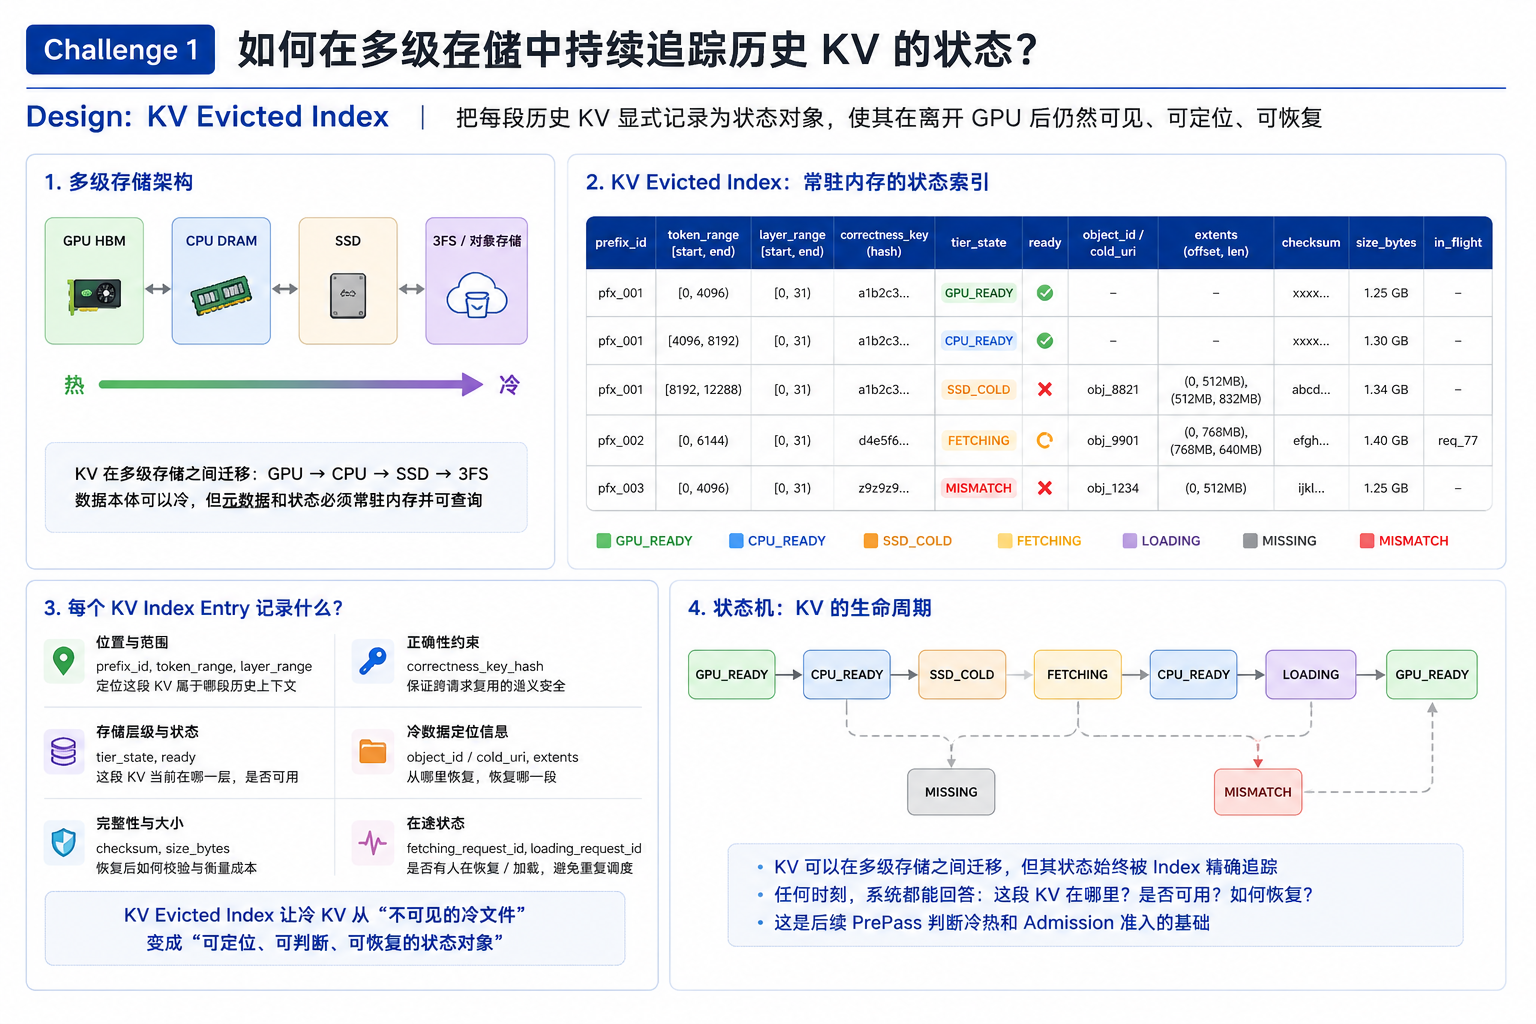
\includegraphics[
    width=1.02\paperwidth,
    height=1.02\paperheight,
    keepaspectratio
  ]{Challenge1.png}
};
\end{tikzpicture}
\end{frame}

\begin{frame}[plain]
\begin{tikzpicture}[remember picture,overlay]
\node at (current page.center) {
  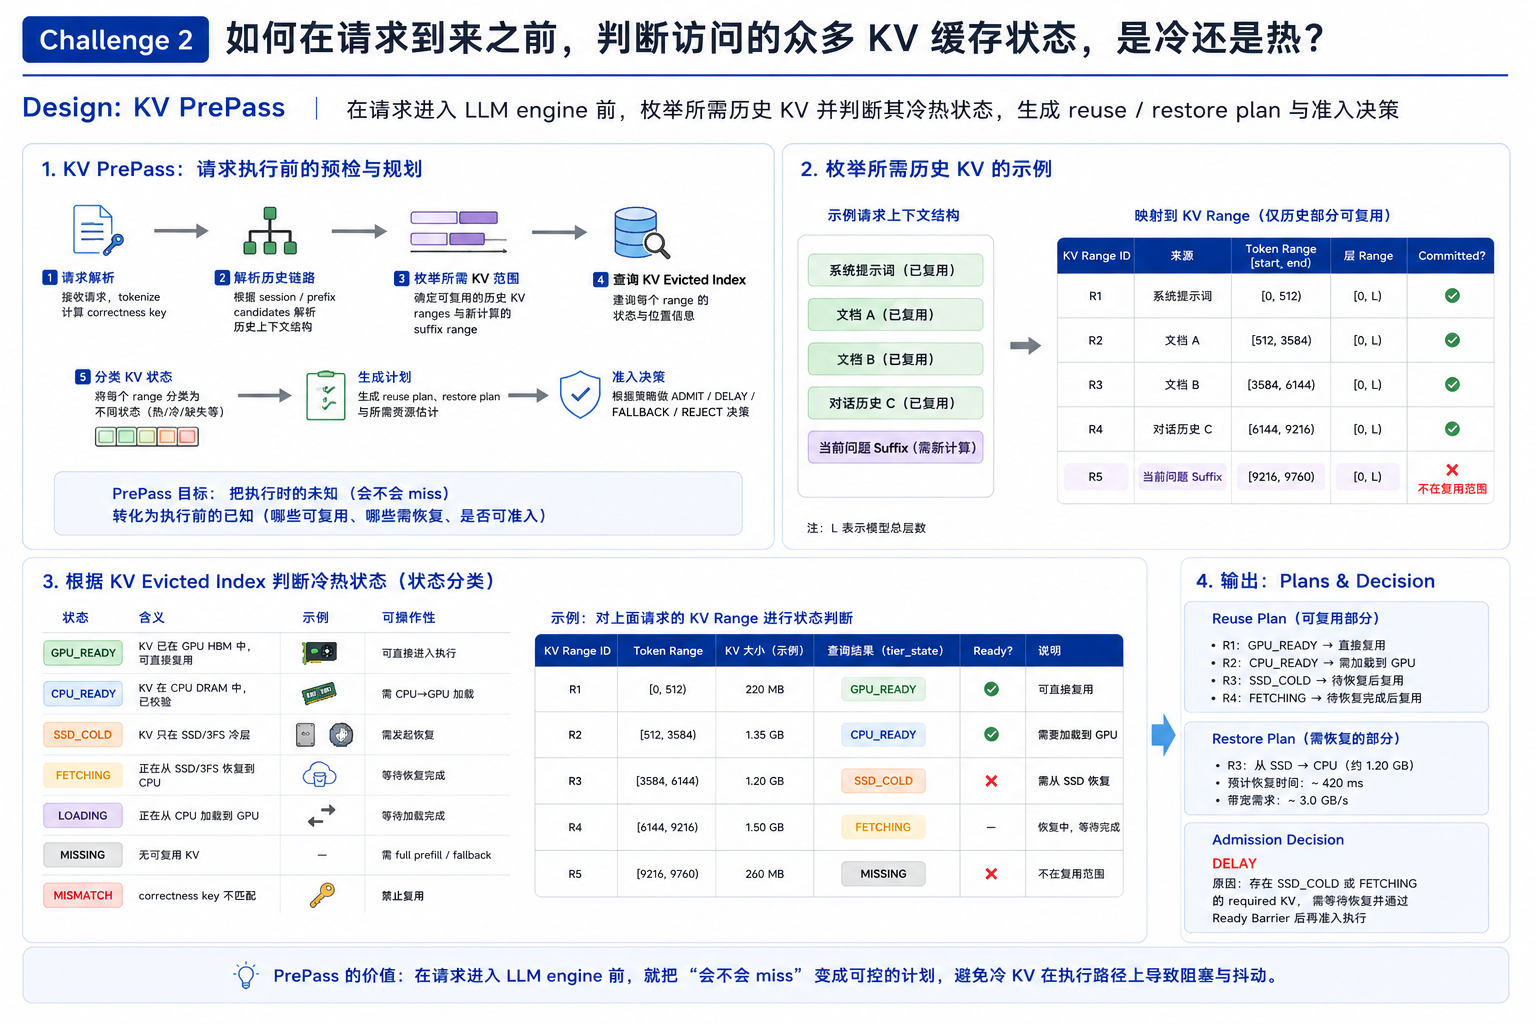
\includegraphics[
    width=1.02\paperwidth,
    height=1.02\paperheight,
    keepaspectratio
  ]{Challenge2.png}
};
\end{tikzpicture}
\end{frame}

\begin{frame}[plain]
\begin{tikzpicture}[remember picture,overlay]
\node at (current page.center) {
  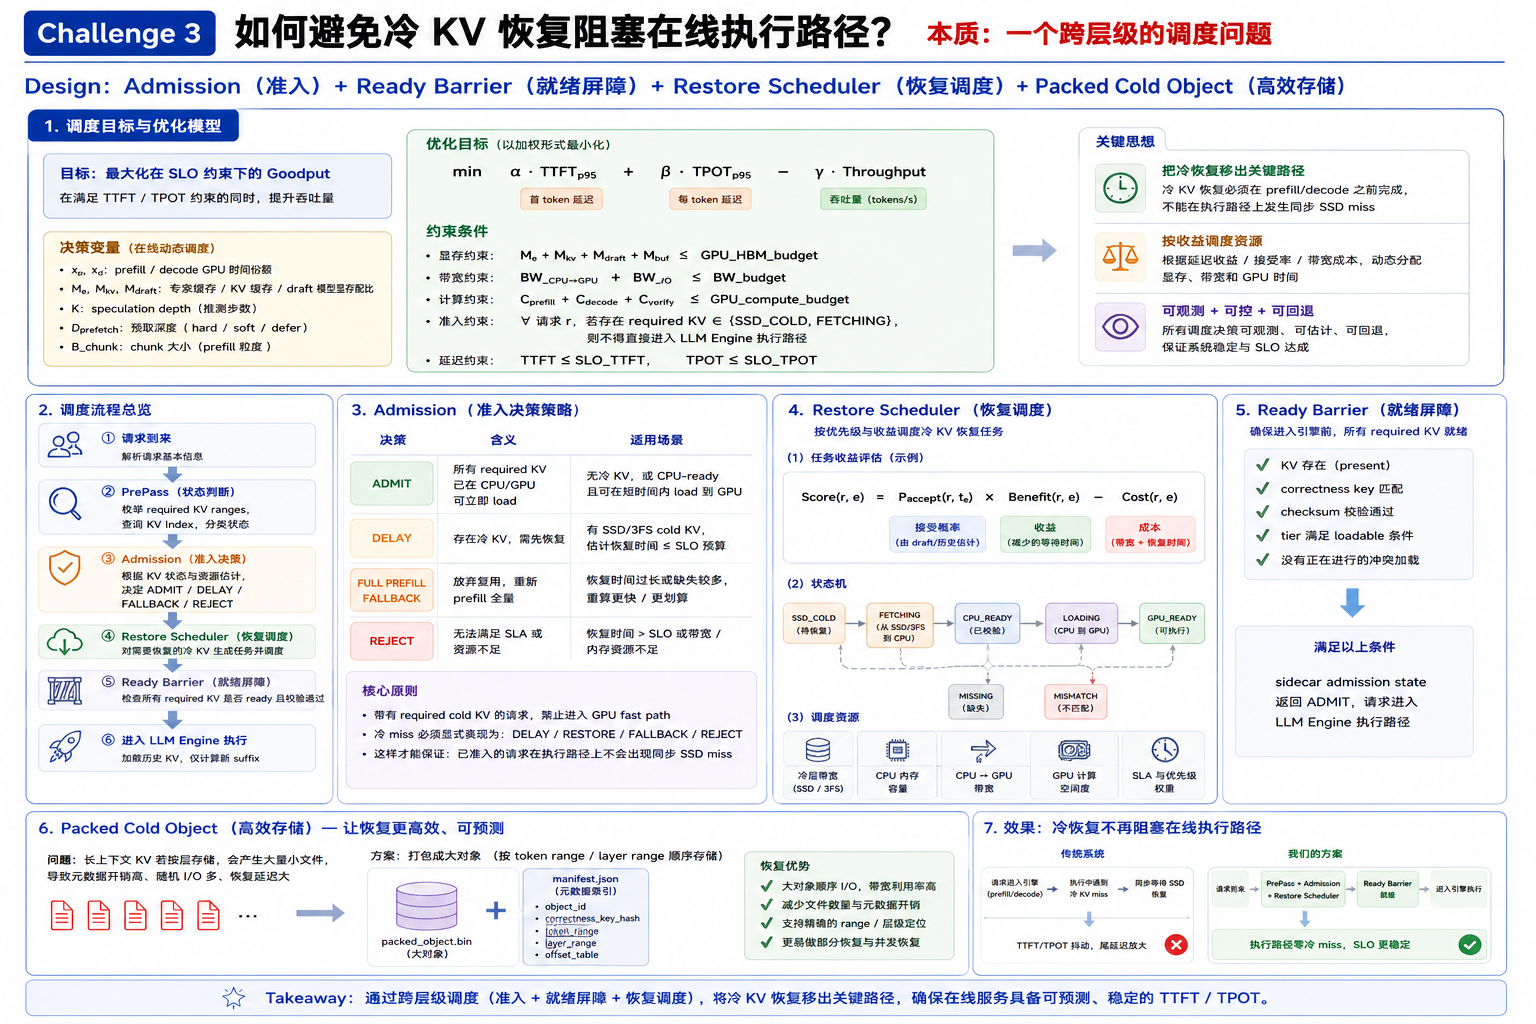
\includegraphics[
    width=1.02\paperwidth,
    height=1.02\paperheight,
    keepaspectratio
  ]{Challenge3.png}
};
\end{tikzpicture}
\end{frame}


% \begin{frame}[t]{我们的设计是什么？(1/3) 持续追踪历史 KV 状态}
% \scriptsize
% \vspace{-0.7em}

% \begin{block}{Challenge 1：如何在多级存储中持续追踪历史 KV 的状态？}
% 历史 KV 会在 HBM、DRAM、SSD/3FS 之间迁移。设计目标是把 KV 从引擎内部的临时缓存，提升为控制面可查询、可校验、可恢复的服务状态。
% \end{block}

% \vspace{0.05em}

% \begin{columns}[T,onlytextwidth]
% \begin{column}{0.49\textwidth}
% \begin{block}{1. KV 范围清单}
% 以 token 范围和层范围作为最小状态单元，为每段 KV 建立持久化描述。
% \begin{itemize}
% \setlength{\itemsep}{0em}
% \item \textbf{身份：}\texttt{session\_id}、轮次、token/层范围。
% \item \textbf{正确性：}模型、分词器、位置编码、数据类型、布局、校验和。
% \item \textbf{位置：}存储层级、对象编号、字节偏移、大小。
% \end{itemize}
% \end{block}
% \end{column}

% \begin{column}{0.49\textwidth}
% \begin{block}{2. 驻留状态机}
% 驻留表记录每段 KV 的实时状态，并约束状态迁移。
% \begin{itemize}
% \setlength{\itemsep}{0em}
% \item \texttt{GPU\_就绪 / CPU\_就绪 / 冷层}。
% \item \texttt{恢复中 / 加载中 / 缺失 / 不匹配}。
% \item 维护版本、引用计数、最近访问时间和恢复代价。
% \end{itemize}
% \end{block}
% \end{column}
% \end{columns}

% \vspace{0.05em}

% \begin{block}{3. 原子提交与降温}
% 请求成功后，连接器先提交 KV 清单、校验和与冷层对象；只有清单提交成功后，系统才释放 HBM/DRAM 副本。降温、恢复、失效都必须先更新驻留表，再向 vLLM 暴露可复用状态。
% \end{block}

% \vspace{0.02em}
% \begin{beamercolorbox}[wd=\linewidth,sep=0.35em,rounded=true]{block body}
% \textbf{\textcolor{AccentRed}{输出：}}
% 对任意历史 KV 范围，控制面都能返回“状态、位置、版本、恢复代价”，为后续预检查与准入控制提供唯一事实来源。
% \end{beamercolorbox}

% \end{frame}

% \begin{frame}[t]{我们的设计是什么？(2/3) 执行前判断所需 KV 冷热}
% \scriptsize
% \vspace{-0.7em}

% \begin{block}{Challenge 2：如何在请求进入 LLM 引擎之前判断其所需 KV 的冷热状态？}
% 一个请求可能只复用长历史中的若干范围。设计目标是在进入 vLLM 前完成所需 KV 枚举、正确性校验和冷热分类，生成明确的复用计划与恢复计划。
% \end{block}

% \vspace{0.05em}

% \begin{columns}[T,onlytextwidth]
% \begin{column}{0.50\textwidth}
% \begin{block}{1. KV 预检查：发现所需范围}
% 网关/旁路控制面在请求准入前执行轻量预检查。
% \begin{itemize}
% \setlength{\itemsep}{0em}
% \item 根据会话脉络和提示前缀定位可复用历史。
% \item 生成本轮所需 token/层范围。
% \item 对齐 vLLM 块/页粒度，避免运行时再拆分。
% \end{itemize}
% \end{block}
% \end{column}

% \begin{column}{0.48\textwidth}
% \begin{block}{2. 正确性与驻留状态探测}
% 预检查查询清单和驻留表，逐段判定能否复用。
% \begin{itemize}
% \setlength{\itemsep}{0em}
% \item 校验模型、分词器、位置编码、数据类型和校验和。
% \item 分类为 \texttt{GPU\_就绪 / CPU\_就绪 / 冷层}。
% \item 标记为 \texttt{恢复中 / 缺失 / 不匹配}。
% \end{itemize}
% \end{block}
% \end{column}
% \end{columns}

% \vspace{0.05em}

% \begin{block}{3. 复用计划与恢复计划}
% 预检查输出两类计划：复用计划描述哪些范围可直接挂接到预填充/解码；恢复计划描述冷层范围的对象编号、偏移、长度、目标层级、截止时间和预计代价。缺失或不匹配的范围直接进入重算或拒绝分支。
% \end{block}

% \vspace{0.02em}
% \begin{beamercolorbox}[wd=\linewidth,sep=0.35em,rounded=true]{block body}
% \textbf{\textcolor{AccentRed}{输出：}}
% 请求进入 LLM 引擎之前，系统已经得到“就绪集合、冷层集合、恢复中集合、降级集合”，避免执行阶段才发现不可复用 KV。
% \end{beamercolorbox}

% \end{frame}

% \begin{frame}[t]{我们的设计是什么？(3/3) 避免冷 KV 阻塞执行路径}
% \scriptsize
% \vspace{-0.7em}

% \begin{block}{Challenge 3：如何避免冷 KV 恢复阻塞在线执行路径？}
% 冷 KV 不能在预填充或解码中同步读取。设计目标是把 SSD/3FS 读写从执行关键路径移到控制面，用预算化恢复、准入控制和就绪屏障保证 vLLM 只消费就绪 KV。
% \end{block}

% \vspace{0.05em}

% \begin{columns}[T,onlytextwidth]
% \begin{column}{0.50\textwidth}
% \begin{block}{1. 预算化恢复调度}
% 调度器把恢复看作有截止时间的多资源任务，而不是后台尽力搬运。
% \begin{itemize}
% \setlength{\itemsep}{0em}
% \item 估计 SSD/3FS 读取、网络、DRAM、主机到显存搬运和 GPU 空闲预算。
% \item 合并相邻冷层范围，并复用正在进行的恢复任务。
% \item 按截止时间、收益和短请求隔离需求排序。
% \end{itemize}
% \end{block}
% \end{column}

% \begin{column}{0.48\textwidth}
% \begin{block}{2. 准入决策}
% 请求进入 vLLM 前必须得到确定结果，而不是带着冷层缺失继续执行。
% \begin{itemize}
% \setlength{\itemsep}{0em}
% \item \texttt{准入}：所需范围已全部就绪。
% \item \texttt{等待}：冷层范围可在首词延迟预算内恢复。
% \item \texttt{降级/拒绝}：预算不足或正确性校验失败。
% \end{itemize}
% \end{block}
% \end{column}
% \end{columns}

% \vspace{0.05em}

% \begin{block}{3. 两阶段就绪屏障}
% 第一阶段在预填充复用前检查历史 KV 是否就绪；第二阶段在解码前确认后续访问不会触发同步冷层缺失。若任一范围恢复失败、版本变化或超时，请求回到 KV 预检查重新规划，而不是进入执行后等待 I/O。
% \end{block}

% \vspace{0.02em}
% \begin{beamercolorbox}[wd=\linewidth,sep=0.35em,rounded=true]{block body}
% \textbf{\textcolor{AccentRed}{输出：}}
% 准入后的 vLLM 只加载就绪 KV；系统以“同步冷层缺失次数为零”为协议约束，稳定避免冷层读写暴露到预填充/解码路径。
% \end{beamercolorbox}

% \end{frame}

\begin{frame}[t]{System Overview: KV Anti-Caching 控制闭环}
\scriptsize
\vspace{-0.6em}

\centering
\resizebox{\linewidth}{!}{%
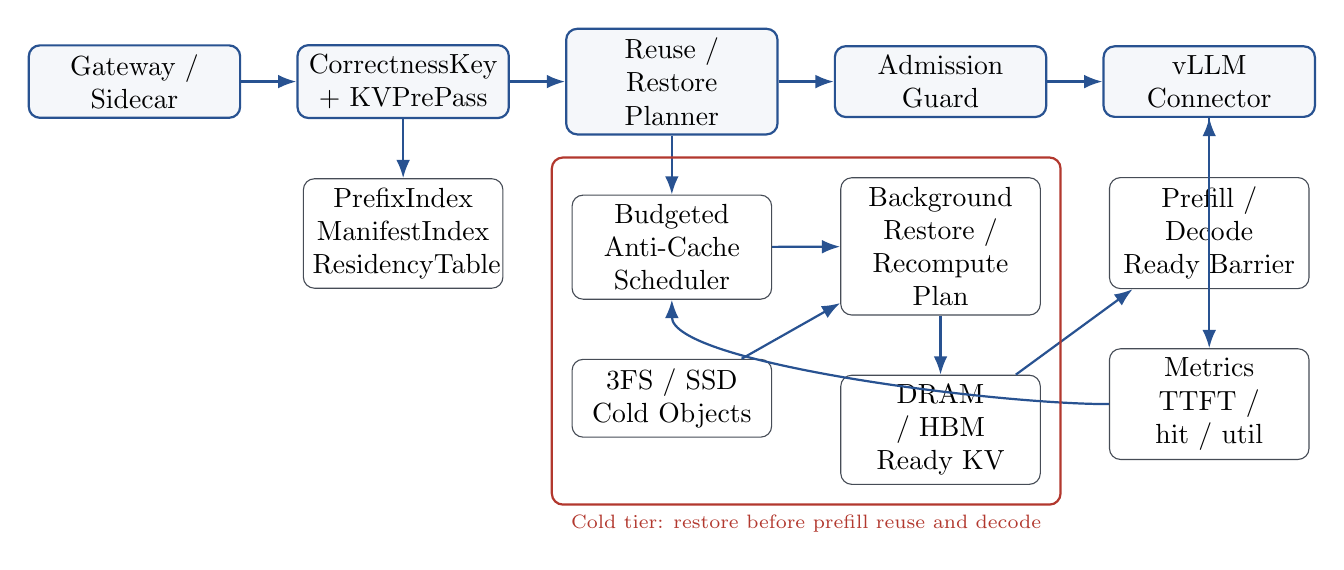
\begin{tikzpicture}[
  node distance=0.55cm and 0.7cm,
  box/.style={draw=MainBlue, thick, rounded corners, fill=SoftGray, align=center, minimum height=0.75cm, text width=2.45cm},
  smallbox/.style={draw=DarkGray, rounded corners, fill=white, align=center, minimum height=0.65cm, text width=2.3cm},
  arrow/.style={-Latex, thick, draw=MainBlue}
]
\node[box] (gateway) {Gateway /\\ Sidecar};
\node[box, right=of gateway] (prepass) {CorrectnessKey\\ + KVPrePass};
\node[box, right=of prepass] (planner) {Reuse / Restore\\ Planner};
\node[box, right=of planner] (admission) {Admission\\ Guard};
\node[box, right=of admission] (vllm) {vLLM\\ Connector};

\node[smallbox, below=0.75cm of prepass] (index) {PrefixIndex\\ ManifestIndex\\ ResidencyTable};
\node[smallbox, below=0.75cm of planner] (sched) {Budgeted\\ Anti-Cache\\ Scheduler};
\node[smallbox, below=0.75cm of admission] (exec) {Background\\ Restore /\\ Recompute Plan};
\node[smallbox, below=0.75cm of vllm] (barrier) {Prefill / Decode\\ Ready Barrier};

\node[smallbox, below=0.75cm of sched] (cold) {3FS / SSD\\ Cold Objects};
\node[smallbox, below=0.75cm of exec] (dram) {DRAM / HBM\\ Ready KV};
\node[smallbox, below=0.75cm of barrier] (metrics) {Metrics\\ TTFT / hit / util};

\draw[arrow] (gateway) -- (prepass);
\draw[arrow] (prepass) -- (planner);
\draw[arrow] (planner) -- (admission);
\draw[arrow] (admission) -- (vllm);
\draw[arrow] (prepass) -- (index);
\draw[arrow] (planner) -- (sched);
\draw[arrow] (sched) -- (exec);
\draw[arrow] (exec) -- (dram);
\draw[arrow] (dram) -- (barrier);
\draw[arrow] (barrier) -- (vllm);
\draw[arrow] (cold) -- (exec);
\draw[arrow] (vllm) -- (metrics);
\draw[arrow] (metrics.west) .. controls +(left:1.5cm) and +(down:0.8cm) .. (sched.south);

\node[draw=AccentRed, thick, rounded corners, fit=(sched)(exec)(cold)(dram), inner sep=0.25cm, label={[text=AccentRed,font=\scriptsize]below:Cold tier: restore before prefill reuse and decode}] {};
\end{tikzpicture}
}

\vspace{0.4em}
\begin{beamercolorbox}[wd=\linewidth,sep=0.55em,rounded=true]{block body}
\textbf{\textcolor{MainBlue}{关键边界：}}
sidecar/control plane 做准入、恢复、fallback 和预算；vLLM connector 只加载已经 ready 的 KV。
\texttt{tier=3FS/SSD} 且 \texttt{ready=false} 的 KV 不能被 prefill reuse 或 decode 同步读取。
\end{beamercolorbox}

\end{frame}

\begin{frame}[t]{What Is the Experiment Plan?}
\footnotesize
\vspace{-0.45em}

\begin{columns}[T,onlytextwidth]
\begin{column}{0.49\textwidth}
\begin{block}{1. 模型与 workload}
\textbf{模型：}
Qwen2.5-14B 作为主线，Qwen3-32B 作为压力上界。

\vspace{0.15em}
\textbf{Workload：}
session append、shared prefix、agent trace、idle restore、mixed short/long、low-locality negative control。
\end{block}
\end{column}

\begin{column}{0.49\textwidth}
\begin{block}{2. 系统与基线}
\textbf{本文系统：} vLLM connector + sidecar + KV Anti-Caching scheduler。

\vspace{0.15em}
\textbf{基线：} vLLM APC、LMCache、naive offload、DualPath-style、Tutti/SSD-backed fast path。
\end{block}
\end{column}
\end{columns}

\vspace{0.2em}

\begin{block}{3. 实验规划}
\begin{itemize}
  \setlength\itemsep{0.03em}
  \item \textbf{端到端性能：}
  TTFT p50/p95/p99、TTFT ratio、ITL、goodput、short-request P99。
  \item \textbf{KV 命中与恢复：}
  historical KV hit rate、byte hit rate、admitted hit rate、useful/restored bytes。
  \item \textbf{冷层与带宽：}
  3FS/NVMe/network/H2D utilization、queue depth、deadline miss、tail latency。
  \item \textbf{规模扩展：}
  从 512/2K/8K/32K 到 128K/1M scaling，分清实机验证与仿真外推。
  \item \textbf{消融实验：}
  去掉 pre-pass、partial promote、budget controller、ready barrier、workload classifier。
\end{itemize}
\end{block}

\end{frame}

\begin{frame}[t]{What Is the Takeaway?}
\small
\vspace{1.0em}

\begin{beamercolorbox}[wd=\linewidth,sep=1.05em,rounded=true]{block body}
\Large
\centering
\textbf{
多轮长上下文服务的关键不只是把 KV 存到更大的存储层级里，而是要将历史 KV 显式管理为可索引、可恢复、可准入控制的持久服务状态，并在请求进入 LLM 引擎前完成冷热判断与恢复调度，从而避免冷 KV 访问破坏在线推理延迟。
}
\end{beamercolorbox}

\end{frame}

\end{document}
